\documentclass[tikz,border=5mm]{standalone}
\begin{document}
	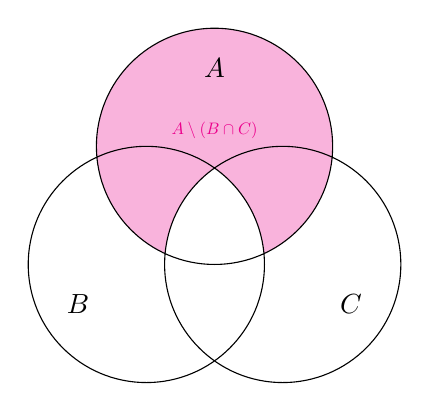
\begin{tikzpicture}
		\def\r{1.5} \def\d{1}
		\def\firstC{(90:\d) circle(\r)}
		\def\secondC{(-30:\d) circle(\r)}
		\def\thirdC{(210:\d) circle(\r)}
		
		\fill[magenta!30] \firstC;   
		\begin{scope}
			\clip \firstC;
			\clip \secondC;
			\fill[white] \thirdC;
		\end{scope}
		\draw \firstC \secondC \thirdC;
		
		\path
		(90:1.2*\d) node[magenta,scale=.6]{$A\setminus (B\cap C)$} 
		(90:2*\d)  node{$A$}
		(210:2*\d) node{$B$}
		(-30:2*\d) node{$C$};
	\end{tikzpicture}
\end{document}